\documentclass[12pt]{article}
\usepackage{amsfonts, epsfig}
\usepackage[authoryear]{natbib}
\usepackage{graphicx}
\usepackage{fancyhdr}
\pagestyle{fancy}
\lfoot{\texttt{comsm0021.github.io}}
\lhead{Neural Information Processing - 8\_forward\_models - Conor}
\rhead{\thepage}
\cfoot{}


\usepackage{tikz}

\usepackage{pgf}
\usepackage[utf8]{inputenc}
\usetikzlibrary{arrows,automata}
\usetikzlibrary{positioning}


\tikzset{
    neuron/.style={
           rectangle,
           rounded corners,
           draw=black, very thick,
           inner sep=2pt,
           text centered,
           },
}



\tikzset{
    area/.style={
           rectangle,
           draw=black, very thick,
           inner sep=2pt,
           text centered,
           },
}


\tikzset{
    gc/.style={
           rectangle,
           rounded corners,
           draw=red, very thick,
           inner sep=2pt,
           text centered,
           },
}


\tikzset{
    inh/.style={
           rectangle,
           rounded corners,
           draw=blue, very thick,
           inner sep=2pt,
           text centered,
           },
}



\tikzset{
    io/.style={
           rectangle,
           draw=green, very thick,
           inner sep=2pt,
           text centered,
           },
}


\begin{document}

\section*{A forward model for the perception of movement}

In neuroscience, and in control theory, a \textsl{forward model} is an
internal model responsible for what performing calculations analagous
to the dead reckoning discussed in the context of Kalman filters.

A well-known discussion of forward models in given in
\cite{WolpertEtAl1995}. In this paper they give some, albeit quite
circumstantial, evidence that the brain has a forward model for
movement. In their experiment subjects are sat in the dark with one
hand on a manipulandum, that is, a device you push around with one
hand which can record your hand, restrict it to specific paths and
excert a force against or with the movement of your hand. A
manipulandum is shown in Fig.~\ref{fig_manipulandum}.

In this experiment the manipulandum is restricted to horizonal
motion. At the start of each trial the location of the subjects hand
is illuminated and it is assumed that at that time the subject knows
exactly where their hand is. The subject is then asked to move their
hand; there may be a force assisting or resisting this movement, in
any case at the end a restiance force is used to force the subject to
stop moving there hand at a point uniformly chosen between zero and 30
cm.  The subject is then asked to use their other hand to indicate,
using a mouse which moves a marker along the horizonal track, where
they believe where their hand is. It turns our people consistiently
over-estimate how far their hand has travelled.\footnote{This raises a
  plethora of questions; like if they then get visual feedback does
  the estimate improve? Is the overestimate the result of not
  modelling the braking force? This isn't dealt with in the paper and
  may work against its conclusions!}  In fact this overestimate has a
distinctive timecourse shown in Fig.~\ref{fig_overestimate}: the
overestimate increases rapidly for movements that take a second or
less and then descreases slowly for longer movements.


\begin{figure}
\begin{center}
  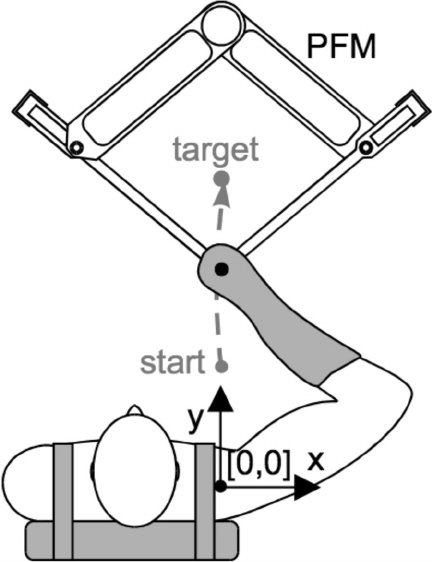
\includegraphics[width=6cm]{manipulandum.jpg}
\end{center}
\caption{A manipulandum allows hand movements to be recorded and to be
  manipulated by applying a force. [Image from \cite{MistryEt2013},
    the start and target labels don't apply to the experiment being
    discussed here].\label{fig_manipulandum}}
\end{figure}


\begin{figure}
\begin{center}
  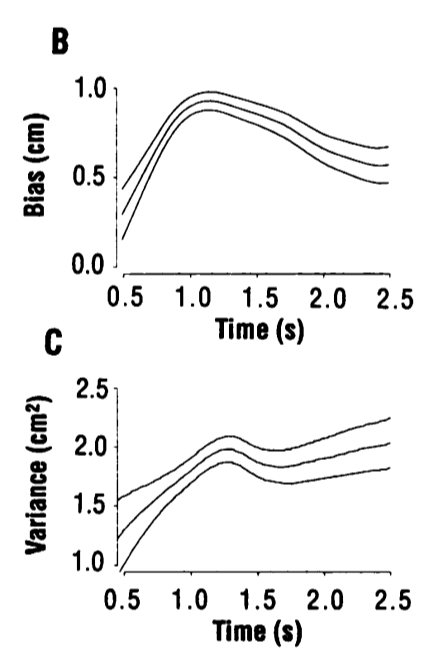
\includegraphics[width=5cm]{fig_overestimate.png}
\end{center}
\caption{The bias in estimates of hand position; \textbf{B} shows the
  mean bias and \textbf{C} the mean variance. The middle line shows
  the mean and the two outer lines are standard errors indicating the
  variability of the measurement. The participants never stop moving
  their hands in less than 0.5 seconds so the graphs start there;
  after 2.5 second the bias stops changing; 1 second corresponds to
  0.9 cm and 2.5 seconds to 2 cm. It should be noted that this is only
  a small fraction of the trials, the trials themselves are uniformly
  chosen from between zero and 30cm, we are told the result plateaus after 2.5 seconds. [Image from
    \cite{WolpertEtAl1995}].\label{fig_overestimate}}
\end{figure}

It is proposed in \cite{WolpertEtAl1995} that this is evidence for a
forward model. In there description the sense of hand position in the
absence of visual feedback has two components, a dead reckoning
component supplied by the forward model and a proprioceptive component
coming from mechano-receptors and joint receptors in the arm
itself. The dead reckoning model is similar to what we saw before for
the Kalman filter:
\begin{equation}
\mathbf{x}_d=F\textbf{x}+U(t)\textbf{c}+\textbf{W}
\end{equation}
where, as before 
\begin{equation}
F=\left(\begin{array}{cc}1&t\\0&1\end{array}\right)
\end{equation}
but here there is in addition a control vector corresponding to the
force the subject applies to the manipulandum. 
\begin{equation}
\textbf{c}=\left(\begin{array}{c} 0\\1/m\end{array}\right)
\end{equation}
and $U(t)$ is the work done on the manipulandum, so $U(t)=\int_0^t
u(t)dt$ where $u(t)$ is the force on the manipulandum, both from the
subject and, possibiliy, from the added force applied to the
manipulandum during the experiment. Finally $\textbf{W}$ is the
noise. Basically, the difference from what we saw before is the extra
control term modelling the accelleration of the manipulandum. In this
picture this force is something the brain knows about, they are the
motor commands whose effect is begin modelled. In any case, the
details here are not important, the main thing is that in this model
the brain models the consequence of the motor commands and produces a
prediction based on dead reckoning of where the hand is. One detail is
important, the covariance of $\mathbf{W}$ grows with time, if $W$ is
the covariance matrix then $W=wt$ for some $w$.

Overall the model has a prediction from the forward model and sensory
information from proprioception; these are combined to give a new
estimate of the position $\mathbf{x}_n$
\begin{equation}
\mathbf{x}_n=\textbf{x}_d+K(\textbf{x}_s-\textbf{x}_d)
\end{equation}
where $\mathbf{x}_s$ is the sensory estimate of the position and $K$
is the Kalman gain.\footnote{All this is described in position space,
  as if in the brain the sensory information is converted into
  position information; a more likely picture is that the forward
  model outputs a sensory prediction. However, this doesn't change the
  picture being presented here.}

In this picture of motor control the movement of the hand is under
continuous feedback control; as the hand is moving the forward model
is predicting where the hand will soon be so the motor areas can issue
instructions for what the muscles must do next to move from that point
to the one beyond. This continuous feedback is a more adaptable and
robust model of motor control than one involving a backward model; in
a backward model the desired final location of the hand is the input
and the output is the required motor commands. 

An additional advantage of a forward model is that it can help with
sensory perception; if there is a prediction of how the sensory
consequence of a model command then this can be used to separate the
expected sensation from the unexpected. Some aspect of the unexpected
sensation will, of course, be attributable to errors in the forward
model, but some will be related to the environment. In fact, there is
a complicated story here, the brain uses differences between the
forward model and the sensory perception to correct its understanding
of, in this case, the hand's location, it uses it to improve sensory
perception of the environment and it uses it to correct the forward
model itself. How it balances these different aspects based on how
often an error occurs and the information, encoded in neuromodulation,
of which is likely to be appropriate, is an interesting open question.


\begin{figure}
\begin{center}
  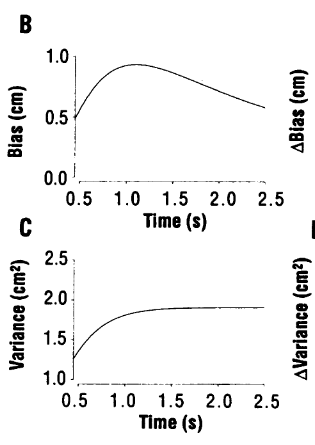
\includegraphics[width=5cm]{fig_model.png}
\end{center}
\caption{The model bias in estimates of hand position; \textbf{B}
  shows the mean bias and \textbf{C} the mean variance. These show
  some similarity to the experimental results; it is clear though that
  the Kalman model doesn't show a plateau as with the experimental
  result unless it is assumed the sensory result, like the dead
  reckoning result, has a bias, just a smaller one and one that
  doesn't grow with movement. [Image from
    \cite{WolpertEtAl1995}].\label{fig_model}}
\end{figure}


Lets return to the experiment. In a Kalman filter the size of the
Kalman gain depends on the variance in the two estimates. If the
variance in the dead reckoning estimate is low compared to the
variance in the sensory estimate then the Kalman gain is near zero;
conversely if the dead reckoning variance is large compared to the
sensory variance the gain is near one. In the authors' account of
their experimental result they imagine that because of the conditions
of the experiment the dead reckoning estimate has a positive bias
which increases with movement.\footnote{There is no explanation as to
  why this might be; this is a weakness of the analysis.} The effect
of this bias is seen in the overestimate. However, the Kalman gain
increases over time; the variance in the dead reckoning estimate
starts at zero and increases, again getting larger and larger with
movement, and so the estimate of the position becomes more and more
reliant on the sensory estimate as time passes, so the bias
reduces. In fact the result of the Kalman filtering model is seen in
Fig.~\ref{fig_model} and gives a good qualitative agreement with
experiment. The key point is that the bias stops in increasing because
the Kalman gain orchestrates a switch from the dead reckoning estimate
to the sensory estimate.

\subsection*{The cerebellum}

This leaves open the question as to where the forward model might be
maintained. The obvious answer is the cerebellum.


\begin{figure}
\begin{center}
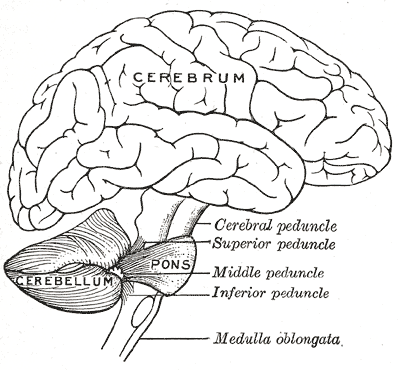
\includegraphics[width=5cm]{fig_gray.png}
\end{center}
\caption{A drawing showing where the cerebellum is in the brain. [Picture from wikipedia which in turn got it from an old edition of \textsl{Gray's Anatomy}]\label{fig_gray}}
\end{figure}


The cerebellum is found at the back of the brain, see
Fig.~\ref{fig_gray}; it is well conserved across vertebrate species
and is known to be involved in movement. The cerebellum has a number
of striking features; it has a more stereotypical structure than most
brain area and this structure is conaerved across species. It also has
one of the brain's largest cells, the Purkinje cell, and its most
numerous, the granule cell.

\begin{figure}
\begin{center}
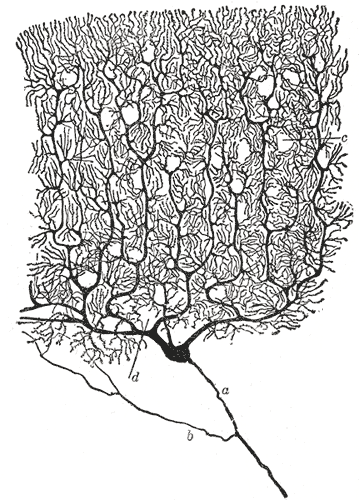
\includegraphics[width=7cm]{Purkinje_cell_by_Cajal.png}
\end{center}
\caption{A drawing by Santiago Ram\'{o}n y Cajal of a Purkinje cell. [Picture taken from \texttt{http://en.wikipedia.org/wiki/Golgi's\_method}]\label{fig:PC}}
\end{figure}

Purkinje cells have a distinctive structure with a huge, highly
branched, but flat dendritic arbor, see Fig.~\ref{fig:PC}; this allows
an extensive connectivity with each Purkinje cell receiving inputs
from around 100,000 other cells. In the cerebellum the Purkinje cell
are lined up like pages in a book, with their arbors lying in parallel
planes. They receive two excitatory inputs, weak inputs from parallel
fibres, axons that run perpendicular to the planes of the Purkinje
cell dendritic arbors, and a strong input from a climbing fibre, a
single axon which winds around the Purkinje cell and makes multiple
contacts with it, see Fig.~\ref{fig:cerebellum}.

\begin{figure}
\begin{center}
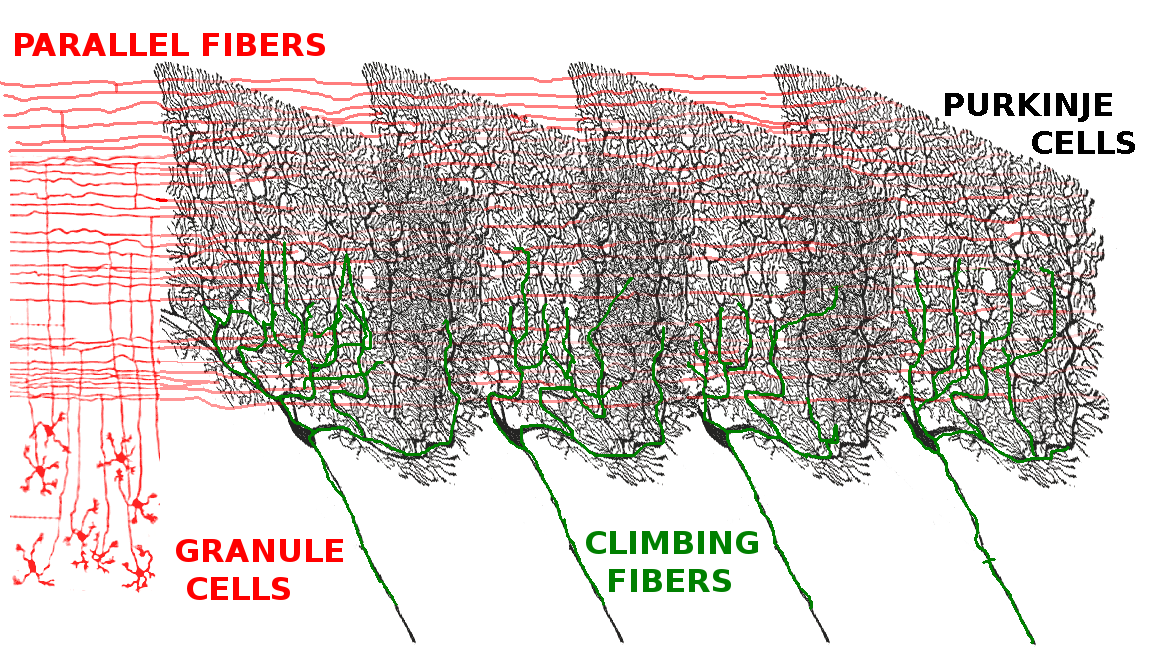
\includegraphics[width=11cm]{cerebellum.png}
\end{center}
\caption{A cartoon of the cerebellar circuitary. A vertical axon rises
  from each granule cells, splits once and then extends horizontally
  in two directions making connections with multiple Purkinje
  cells. Each Purkinje cell has its own climbing fiber which winds up
  around it.\label{fig:cerebellum}}
\end{figure}


\begin{figure}
\begin{center}
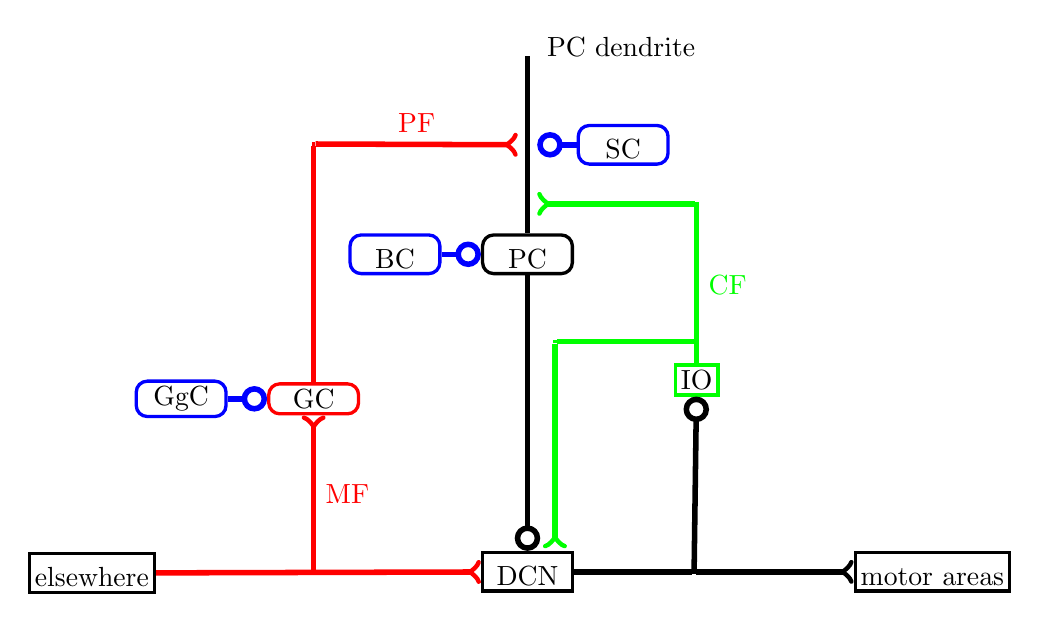
\begin{tikzpicture}
\node[neuron,text width=1cm, text height=0.35cm](PC){PC};
\node[inh,text width=1cm, text height=0.35cm,left = 0.5cm of PC](BC){BC};
\node[above = 1cm of PC](PCd){};
\node[inh,text width=1cm, text height=0.35cm,right = 0.5cm of PCd](SC){SC};
\node[above = 0.25cm of PC](PCc){};
\node[scale = 0.2,fill=green,right = 2cm of PCc](PCcr){};
\node[above = 1cm of PCd](PCdd){};
\node[right = 0cm of PCdd](){PC dendrite};
\node[left = 2cm of PC](PCl){};
\node[gc,text width=1cm,below = 1.5cm of PCl](GC){GC};
\node[inh,text width=1cm,left = 0.5cm of GC](GgC){GgC};
\node[scale = 0.2,fill=red,above = 3cm of GC](GCa){};
\node[scale = 0.01,fill=red,below = 2cm of GC](GCb){};
\node[io,below = 2cm of PCcr](IO){IO};
\node[scale =0.2,fill=green,above = 0.25cm of IO](IOa){};
\node[scale =0.2,fill=green,left = 1.75cm of IOa](IOl){};
\node[scale =0.01,below = 2.6cm of IOl](IOlb){};
\node[area,text width=1cm, text height=0.35cm,below  = 3.5cm of PC](DCN){DCN};
\node[scale=0.2,fill=black,right= 1.5cm of DCN](DCNr){};
\node[area,text height=0.35cm,right = 2cm of DCNr](ma){motor areas};
\node[area,text height=0.35cm,left = 2cm of GCb](ew){elsewhere};
\path (PCdd) edge[-,line width=2pt](PC);
\path (PC) edge[-o,line width=2pt] (DCN);
\path (IO) edge[-,green,line width=2pt] node[anchor=west]{CF} (PCcr);
\path (PCcr) edge[-<,green,line width=2pt] (PCc);
\path (GC) edge[-,red,line width=2pt] (GCa);
\path (GCa) edge[-<,red,line width=2pt] node[anchor=south]{PF}(PCd);
\path (GCb) edge[-<,red,line width=2pt] node[anchor=west]{MF} (GC);
\path (ew) edge[-<,red,line width=2pt] (DCN);
\path (DCN) edge[-,black,line width=2pt] (DCNr);
\path (DCNr) edge[-o,black,line width=2pt] (IO);
\path (DCNr) edge[-<,black,line width=2pt] (ma);
\path (IOa) edge[-,green,line width=2pt](IOl);
\path (IOl) edge[-<,green, line width=2pt](IOlb);
\path (GgC) edge[-o,blue, line width=2pt](GC);
\path (BC) edge[-o,blue, line width=2pt](PC);
\path (SC) edge[-o,blue, line width=2pt](PCd);
\end{tikzpicture}
\end{center}
\caption{A schematic of the cerebellar circuit. The granule cells (GC)
  receive input from a diverse range of other parts of the brain along
  the mossy fibers (MF). Each granule cell will combine input from
  just three or four mossy fibers and do this in lots of different
  combinations. The parallel fiber (PF) carries spikes from the GC to
  the Purkinje cell (PC) whose large dendrite is drawn as a line. The
  PC also receives input from a climbing fiber (CF) coming from
  Inferior Olivary Nucleus (IO). In turn it sends an inhibitory signal
  to the Deep Cerebellar Nucleus (DCN); the DCN has inhibitory neurons
  which act on IO and excitatory neurons which act on the motor
  system. The basket cells (BC), the Golgi cells (GgC) and the
  stellate cells (SC) are all local inhibitory
  cells.\label{fig:connectivity}}
\end{figure}

Another peculiarity is that the Purkinje cell has different responses
to different inputs; in response to multiple weak inputs from the
parallel fibers it fires a normal sort of spike, called in this
context a \textsl{simple spike}; in response to single spike from the
climbing fiber is fires a special spike, called a \textsl{complex
  spike}, with a leading spike, a number of small \lq{}spikelets\rq{}
and a sustained after-period of depolarization; this is illustrated in
Fig.~\ref{fig:spikes}.

\begin{figure}
\begin{center}
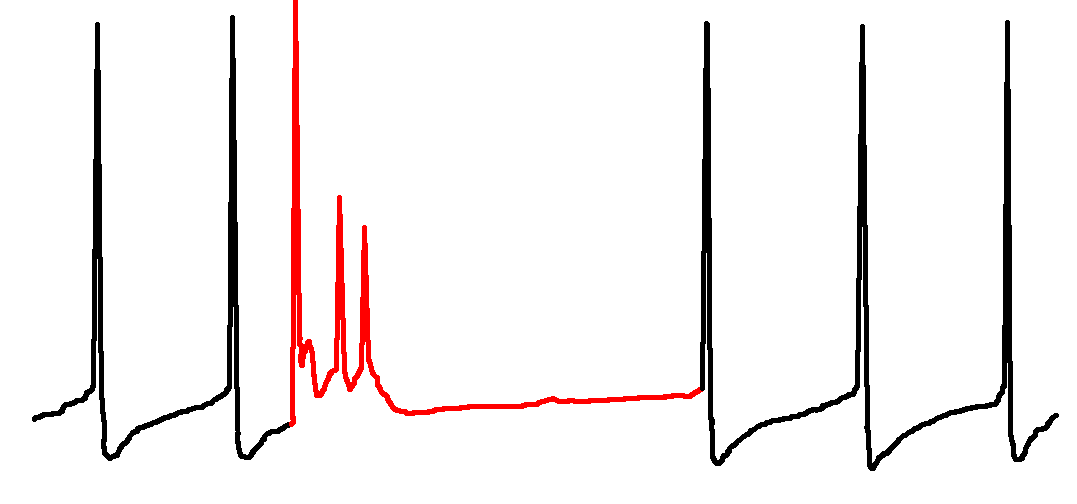
\includegraphics[width=8.cm]{complex_spike.png}
\end{center}
\caption{A complex spike. This drawing shows a simple spikes in black
  and a complex spike in red. The complex spike is followed by a long
  refractory period during which spiking is not possible. This is a
  sketch, not an actual recording, but a typical time scale would have
  this refractory period 50 ms long.\label{fig:spikes}}
\end{figure}

If there is a forward model it seems likely to be supported by the
cerebellum \citep{GaoEtAl1996}. The cerebellum receives input from the motor areas. The
Purkinje cells receive a huge number of input and so appear to be
capable of calculations akin to large matrix multiplications. Finally,
the Purkinje cell has a second input type and this is thought to
communicate an error signal allowing the cerebellum to perform
supervised learning, in other words there seems to be a mechanism for
updating the forward model \citep{Marr1969,Albus1971}.



\bibliographystyle{apa} \bibliography{../../source/bibliography}{}



\end{document}

